\documentclass[../../dis.tex]{subfiles}
\begin{document}
\chapter{L4 - The Storage Layer \& Buffer Management}\label{chap:l4}\vfill
\section{The storage hierarchy}
A DBMS does not operate on one uniform memory. Data moves across a hierarchy of storage levels with very different latency, capacity, and cost.

\begin{dashlist}
    \item \textbf{CPU registers, caches, DRAM}: volatile, byte-addressable, and very fast.
    \item \textbf{SSD, HDD, network storage}: persistent, block-addressable, much larger, and much slower.
    \item Going \emph{up} the hierarchy gives lower latency but less capacity and a higher cost per byte; going \emph{down} gives the opposite.
\end{dashlist}

Main memory holds the \textbf{working set}: the data currently being processed. Persistent storage holds the full database. Modern hardware adds intermediate levels such as \textbf{persistent memory} and \textbf{fast network storage}. Still, the DBMS must move pages carefully between storage and RAM.

\begin{dbtable}{Typical latency numbers}{lcc}
\textbf{Operation} & \textbf{Latency} & \textbf{If 1 ns were 1 s} \\ \hline
L1 cache reference & 1 ns & 1 s \\ \hline
L2 cache reference & 4 ns & 4 s \\ \hline
DRAM access & 100 ns & 100 s \\ \hline
SSD access & 16{,}000 ns & 4.4 h \\ \hline
HDD access & 2{,}000{,}000 ns & 3.3 weeks \\ \hline
Network storage & $\sim 50{,}000{,}000$ ns & 1.5 years \\ \hline
Tape archive & 1{,}000{,}000{,}000 ns & 31.7 years \\
\end{dbtable}

The exact values vary by hardware, but the orders of magnitude do not: one extra I/O can cost more than millions of CPU instructions.

\newpage
\section{Why DBMSs still care about disks}
A DBMS usually keeps only the actively used data in RAM and stores the database itself on secondary storage. This creates two expensive operations:

\begin{dashlist}
    \item \textbf{read}: transfer a page from disk to main memory,
    \item \textbf{write}: transfer a modified page from main memory back to disk.
\end{dashlist}

Relative to in-memory operations, both are expensive, so the DBMS must plan I/O carefully.

\subsection{Why not keep everything in main memory?}
\begin{dashlist}
    \item \textbf{Cost}: large production databases can reach the TB or PB scale, so all-DRAM storage is expensive.
    \item \textbf{Volatility}: conventional DRAM loses data on power failure, but databases need persistence across runs.
    \item \textbf{Main-memory DBMSs}: useful for smaller or latency-critical workloads; larger memories and non-volatile devices make them increasingly practical.
\end{dashlist}

For general-purpose systems, disks remain the default place to store data.

\subsection{Pages and storage devices}
Data is stored and retrieved in units called \textbf{pages} (or \textbf{disk blocks}), not byte by byte.

\begin{concept}{Page (disk block)}\label{def:diskpage}
The basic unit of transfer between secondary storage and main memory. DBMS I/O is organized around whole pages.
\end{concept}

Access cost depends on both the device and the access pattern:
\begin{dashlist}
    \item \textbf{magnetic disks (HDDs)}: very large capacity and low cost per byte, but slow random access; good streaming throughput.
    \item \textbf{flash storage (SSDs)}: lower latency and strong random-read performance, but still far slower than DRAM and more constrained on writes.
    \item \textbf{layout matters}: unlike RAM, page access time depends heavily on where a page is placed and whether access is sequential or random.
\end{dashlist}

\section{Magnetic disk organization}
A magnetic disk stores bits on rotating platters coated with magnetic material. Each disk surface is organized geometrically.\\
\begin{minipage}[htp]{0.62\textwidth}
\begin{concept}{Track}
A concentric circle on one disk surface.
\end{concept}

\begin{concept}{Sector}
A slice of a track and the smallest hardware-addressable unit on the disk.
\end{concept}

\begin{concept}{Cylinder}
The set of tracks at the same radius across all disk surfaces.
\end{concept}
Important details:
\begin{dashlist}
    \item outer tracks are longer, so they can store more sectors and offer higher transfer bandwidth than inner tracks,
    \item disks are divided into \textbf{zones}: all tracks in one zone have the same number of sectors per track,
    \item the hardware exposes a sector-addressable space; common sector sizes are 512 B or 4096 B,
    \item a DBMS page size is a fixed multiple of the sector size,
    \item the main operations are \textbf{read} and \textbf{write}.
\end{dashlist}
\end{minipage}\hfill
\begin{minipage}[htp]{0.36\textwidth}
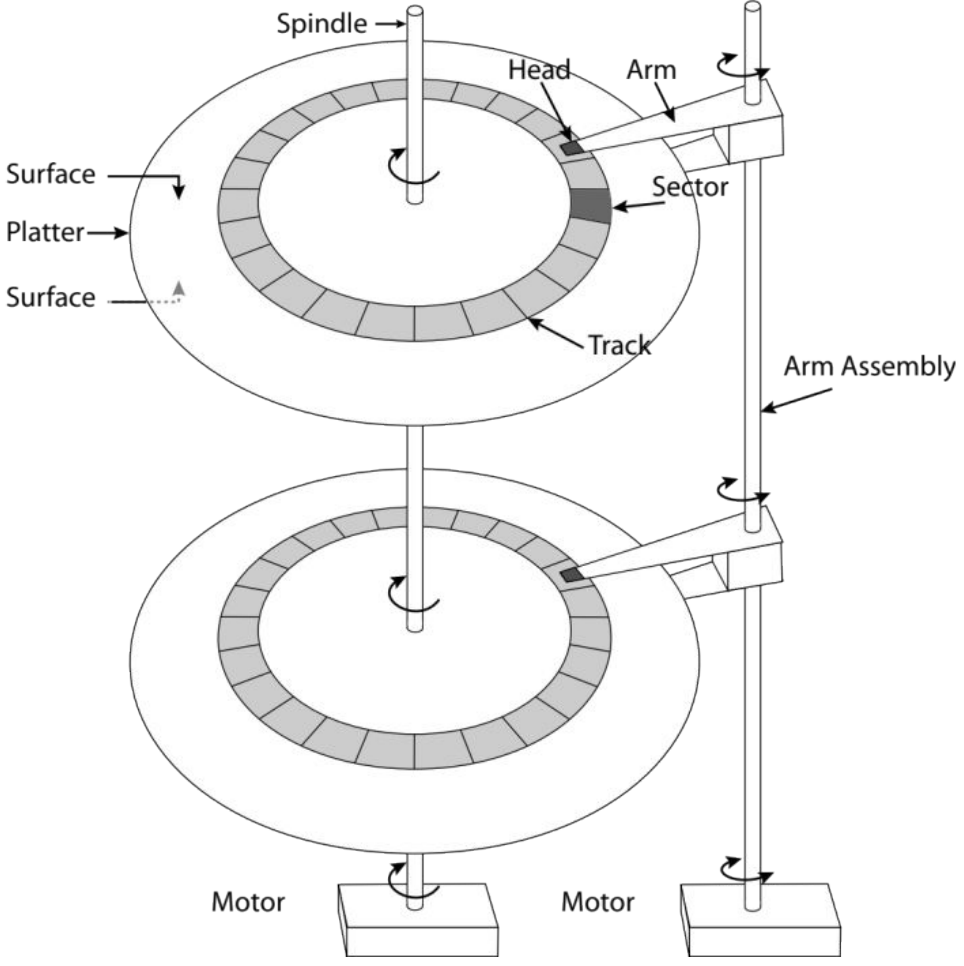
\includegraphics[width=1\textwidth]{images/magnetic.png} 
\end{minipage}

\subsection{Cost of accessing a page}
For a magnetic disk, page access time is well approximated by
\[
\text{access time} = \text{seek time} + \text{rotational delay} + \text{transfer time}.
\]

\begin{concept}{Seek time}
Time to move the disk arm so the head reaches the correct track. Typically, \(5\)--\(15\) ms.
\end{concept}

\begin{concept}{Rotational delay}
Waiting time until the desired sector rotates under the read/write head. At 7200 RPM, one rotation takes about \(8.3\) ms, so the average delay is about half of that.
\end{concept}

\begin{concept}{Transfer time}
Time to actually move the bytes once the head is already in position. For one page, this is usually much smaller than seek and rotation.
\end{concept}

This is why \textbf{sequential access} is much faster than random access: once the head is already near the right place, the DBMS can read neighboring blocks with little extra positioning cost.

\subsection{Arranging pages on disk}
To minimize latency, blocks of the same file should be laid out in a sensible physical order. A good notion of the \textbf{next} block is:

\begin{dashlist}
    \item first, a block on the same track,
    \item then, a block on the same cylinder,
    \item then, a block on an adjacent cylinder.
\end{dashlist}

\begin{concept}{Pre-fetching}
Reading nearby pages before they are explicitly requested, because sequential layout makes them cheap to fetch once the disk is already positioned.
\end{concept}

Physical placement matters a lot: a disk block has several useful physical neighbors, not just one logical successor.

\subsection{A simple disk-performance model}
Assume a magnetic disk with:
\begin{dashlist}
    \item average seek time: \(5\) ms,
    \item spindle speed: \(7200\) RPM \(\Rightarrow\) one rotation in \(\frac{60{,}000}{7200} \approx 8.33\) ms, so average rotational delay \(\approx 4.17\) ms,
    \item transfer rate: \(50\) MB/s,
    \item page size: \(4096\) B \(\Rightarrow\) transfer time \(= \frac{4096}{50 \times 10^6}\,\text{s} \approx 0.082\) ms.
\end{dashlist}

\begin{dbtable}{Example: 4 KB reads on a 7200 RPM HDD}{L{0.47\textwidth}C{0.18\textwidth}C{0.17\textwidth}}
\textbf{Access pattern} & \textbf{Time} & \textbf{Throughput} \\ \hline
Random block anywhere on disk & \(5 + 4 + 0.082 = 9.082\) ms & \(\approx 451\) KB/s \\ \hline
Random block in the same cylinder & \(4 + 0.082 = 4.082\) ms & \(\approx 1.03\) MB/s \\ \hline
Next block on the same track (sequential) & \(0.082\) ms & \(\approx 50\) MB/s \\
\end{dbtable}

The gap is enormous: good physical layout and sequential scans can improve effective bandwidth by two orders of magnitude. Page placement and clustering matter. Buffer management builds on exactly this gap.

\subsection{Rules of thumb}
Two heuristics explain most storage-level design decisions:
\begin{dashlist}
    \item main-memory access is roughly \(\sim 1000\times\) faster than disk I/O,
    \item on magnetic disks, sequential I/O is roughly \(\sim 10\times\) faster than random I/O.
\end{dashlist}

Thus, DBMSs try to keep hot data in memory and lay out pages sequentially on secondary storage.

\section{Flash storage}
Flash memory has existed for decades and evolved from USB keys and mobile-device storage into consumer and enterprise \textbf{SSDs}. In DBMSs, it can serve either as \textbf{main storage} or as an \textbf{accelerator} such as a cache or logging device.

\subsection{Why flash changed storage}
Flash disks are one of the main modern solutions for fast storage:
\begin{dashlist}
    \item they offer orders-of-magnitude higher I/O performance than HDDs,
    \item they expose the same block-oriented API as disks, so DBMSs can still work with pages,
    \item there is no mechanical seek, so \textbf{random reads} are close in cost to \textbf{sequential reads},
    \item unlike HDDs, access time is not determined by physical page location on the device.
\end{dashlist}

\begin{concept}{Flash page and flash block}
Reads and writes operate at \textbf{page} granularity, while erases operate at \textbf{block} granularity. A flash block contains many pages.
\end{concept}

\subsection{Internal organization}
An SSD is a small parallel system rather than a single chip:
\begin{dashlist}
    \item a controller runs firmware and exports a disk-like block interface,
    \item flash packages are connected through \textbf{channels},
    \item each package contains several \textbf{dies} (chips),
    \item each die contains \textbf{planes}, \textbf{blocks}, and \textbf{pages}.
\end{dashlist}

This is why flash access time depends on controller design, internal parallelism, firmware, and package bandwidth, not on a moving disk head. In typical devices, a block may contain dozens of 4 KB pages.

\subsection{Operations, density, and lifetime}
Flash supports three basic operations:
\begin{dashlist}
    \item \textbf{read} and \textbf{write} at page granularity,
    \item \textbf{write} can only program cells from \(1 \rightarrow 0\),
    \item \textbf{erase} resets cells from \(0 \rightarrow 1\), but only at block granularity.
\end{dashlist}

\begin{dbtable}{Common flash families}{lcc}
\textbf{Type} & \textbf{Bits/cell} & \textbf{Typical trade-off} \\ \hline
SLC & 1 & fastest, longest lifetime, highest cost \\ \hline
MLC & 2 & more capacity, lower endurance \\ \hline
TLC & 3 & cheaper per bit, lower endurance and slower writes \\ \hline
QLC & 4 & highest density, lowest endurance; best for read-heavy use \\
\end{dbtable}

As density rises from \textbf{SLC} to \textbf{QLC}, cost per bit falls, but endurance and write performance usually decline. Device lifetime often ranges roughly from \(10^5\) down to \(10^3\) \textbf{program/erase (P/E) cycles}.

\begin{concept}{Wear leveling}
Firmware techniques that spread writes and erases across blocks so that no small region of flash wears out too early.
\end{concept}

\subsection{Flash Translation Layer (FTL)}
\begin{concept}{Flash Translation Layer (FTL)}
The firmware layer that gives SSDs an HDD-like interface. It remaps logical pages to physical flash locations, performs garbage collection, applies wear leveling, and tunes both performance and device lifetime.
\end{concept}

The FTL is necessary because flash cannot overwrite pages in place the way magnetic disks can.

\subsection{Flash versus HDDs}
In practice, the two technologies serve different goals:
\begin{dashlist}
    \item \textbf{HDDs}: best when the main goal is \textbf{large, inexpensive capacity}.
    \item \textbf{Flash}: best when the workload needs \textbf{low latency}, \textbf{high IOPS}, and especially \textbf{efficient random reads}.
\end{dashlist}

\section{Storage requirements and RAID}
Storage systems should ideally be \textbf{fast}, \textbf{reliable}, and \textbf{affordable}. A single disk rarely optimizes all three at once.

\begin{concept}{RAID}
\textbf{R}edundant \textbf{A}rray of \textbf{I}nexpensive \textbf{D}isks. RAID builds one logical disk from several physical disks to improve throughput, reliability, or both.
\end{concept}

RAID combines two main ideas:
\begin{dashlist}
    \item \textbf{striping}: spread data across disks for higher throughput,
    \item \textbf{redundancy}: duplicate or protect data so the array can survive failures.
\end{dashlist}

\subsection{RAID 0: striping}
\begin{dashlist}
    \item file blocks are striped across disks,
    \item there is \textbf{no redundancy}, so RAID 0 provides \textbf{no fault tolerance},
    \item throughput is excellent because the array can use the cumulative bandwidth of all disks,
    \item usable capacity is the sum of the capacities of all disks.
\end{dashlist}

\begin{schema}
{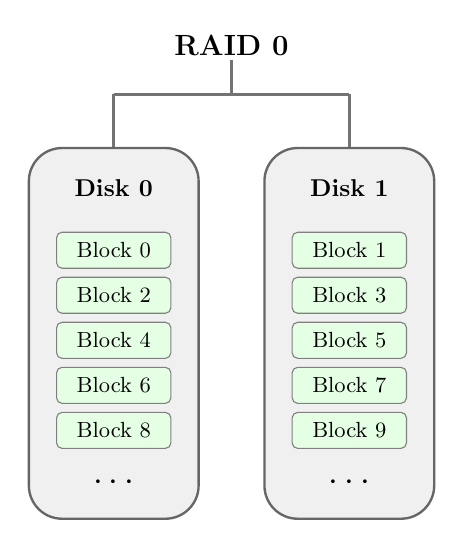
\begin{tikzpicture}[
    x=1cm,y=1cm,
    scale=0.88,
    transform shape,
    every node/.style={font=\small},
    frame/.style={draw=black!60, rounded corners=12pt, line width=0.85pt},
    drive/.style={frame, fill=gray!12, minimum width=2.45cm, minimum height=5.35cm},
    block/.style={draw=black!50, rounded corners=2pt, fill=green!10, minimum width=1.65cm, minimum height=0.52cm},
    bracket/.style={draw=black!55, line width=0.95pt}
]
    \node[font=\bfseries\large] (title) at (1.7,4.15) {RAID 0};
    \draw[bracket] (0,3.45) -- (3.4,3.45);
    \draw[bracket] (0,2.68) -- (0,3.45);
    \draw[bracket] (3.4,2.68) -- (3.4,3.45);
    \draw[bracket] (1.7,3.45) -- (1.7,3.95);

    \node[drive] (d0) at (0,0) {};
    \node[drive] (d1) at (3.4,0) {};
    \node[font=\bfseries] at (0,2.1) {Disk 0};
    \node[font=\bfseries] at (3.4,2.1) {Disk 1};

    \foreach \y/\lab in {1.20/Block 0,0.55/Block 2,-0.10/Block 4,-0.75/Block 6,-1.40/Block 8} {
        \node[block] at (0,\y) {\lab};
    }
    \foreach \y/\lab in {1.20/Block 1,0.55/Block 3,-0.10/Block 5,-0.75/Block 7,-1.40/Block 9} {
        \node[block] at (3.4,\y) {\lab};
    }

    \node[font=\Large] at (0,-2.15) {$\cdots$};
    \node[font=\Large] at (3.4,-2.15) {$\cdots$};
\end{tikzpicture}}\par}
\end{schema}

The downside is reliability: with \(N\) independent disks, the mean time to failure of the striped array is roughly \(\frac{1}{N}\) of the mean time to failure of one disk, because \emph{any} disk failure breaks the array.

\subsection{RAID 1: mirroring}
\begin{dashlist}
    \item every block is duplicated on another disk,
    \item RAID 1 handles \textbf{disk loss} well, but it does \textbf{not} protect against logical corruption or bad writes mirrored to both copies,
    \item usable capacity is only that of one disk per mirror pair,
    \item reads can be parallelized, but each write must update all mirrored copies.
\end{dashlist}

RAID 1 is simple and reliable, but expensive: half of the raw capacity is used for redundancy.

\begin{schema}
{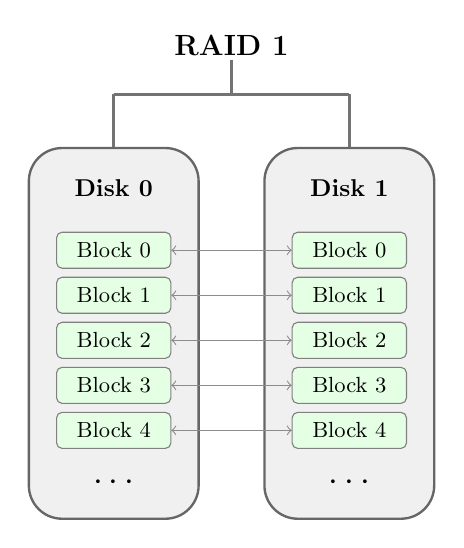
\begin{tikzpicture}[
    x=1cm,y=1cm,
    scale=0.88,
    transform shape,
    every node/.style={font=\small},
    frame/.style={draw=black!60, rounded corners=12pt, line width=0.85pt},
    drive/.style={frame, fill=gray!12, minimum width=2.45cm, minimum height=5.35cm},
    block/.style={draw=black!50, rounded corners=2pt, fill=green!10, minimum width=1.65cm, minimum height=0.52cm},
    bracket/.style={draw=black!55, line width=0.95pt},
    mirror/.style={<->, thin, draw=black!45}
]
    \node[font=\bfseries\large] (title) at (1.7,4.15) {RAID 1};
    \draw[bracket] (0,3.45) -- (3.4,3.45);
    \draw[bracket] (0,2.68) -- (0,3.45);
    \draw[bracket] (3.4,2.68) -- (3.4,3.45);
    \draw[bracket] (1.7,3.45) -- (1.7,3.95);

    \node[drive] (d0) at (0,0) {};
    \node[drive] (d1) at (3.4,0) {};
    \node[font=\bfseries] at (0,2.1) {Disk 0};
    \node[font=\bfseries] at (3.4,2.1) {Disk 1};

    \foreach \y/\lab in {1.20/Block 0,0.55/Block 1,-0.10/Block 2,-0.75/Block 3,-1.40/Block 4} {
        \node[block] at (0,\y) {\lab};
        \node[block] at (3.4,\y) {\lab};
    }

    \foreach \y in {1.20,0.55,-0.10,-0.75,-1.40} {
        \draw[mirror] (0.83,\y) -- (2.57,\y);
    }

    \node[font=\Large] at (0,-2.15) {$\cdots$};
    \node[font=\Large] at (3.4,-2.15) {$\cdots$};
\end{tikzpicture}}\par}
\end{schema}

\subsection{RAID 5: striping with rotating parity}
\begin{concept}{Parity}
An extra block computed as the bitwise XOR of several data blocks. If one block is missing, it can be reconstructed from the parity block and the surviving data blocks.
\end{concept}

For one stripe group,
\[
P = S_0 \oplus S_1 \oplus \cdots \oplus S_{N-2}.
\]

\begin{dashlist}
    \item data is striped across disks, but parity blocks rotate from disk to disk,
    \item the array can survive the loss of \textbf{one} disk,
    \item usable capacity is the equivalent of \(N-1\) disks out of \(N\),
    \item reads are fast, but writes are more complex because parity must be updated.
\end{dashlist}

RAID 5 is a common compromise: it is more affordable than mirroring, more reliable than pure striping, and widely used in servers and datacenters.

\begin{schema}
{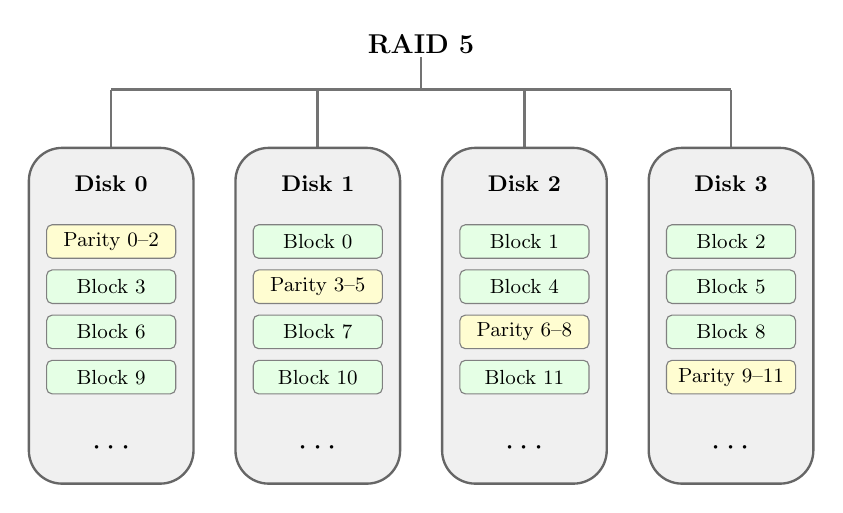
\begin{tikzpicture}[
    x=1cm,y=1cm,
    scale=0.82,
    transform shape,
    every node/.style={font=\small},
    frame/.style={draw=black!60, rounded corners=12pt, line width=0.85pt},
    drive/.style={frame, fill=gray!12, minimum width=2.55cm, minimum height=5.20cm},
    block/.style={draw=black!50, rounded corners=2pt, fill=green!10, minimum width=2.0cm, minimum height=0.52cm},
    parity/.style={draw=black!50, rounded corners=2pt, fill=yellow!18, minimum width=2.0cm, minimum height=0.52cm},
    bracket/.style={draw=black!55, line width=0.95pt}
]
    \node[font=\bfseries\large] (title) at (4.8,4.20) {RAID 5};
    \draw[bracket] (0,3.50) -- (9.6,3.50);
    \foreach \x in {0,3.2,6.4,9.6} {
        \draw[bracket] (\x,2.60) -- (\x,3.50);
    }
    \draw[bracket] (4.8,3.50) -- (4.8,4.00);

    \foreach \x/\name in {0/Disk 0,3.2/Disk 1,6.4/Disk 2,9.6/Disk 3} {
        \node[drive] at (\x,0) {};
        \node[font=\bfseries] at (\x,2.05) {\name};
        \node[font=\Large] at (\x,-2.05) {$\cdots$};
    }

    \node[parity] at (0,1.15) {Parity 0--2};
    \node[block] at (3.2,1.15) {Block 0};
    \node[block] at (6.4,1.15) {Block 1};
    \node[block] at (9.6,1.15) {Block 2};

    \node[block] at (0,0.45) {Block 3};
    \node[parity] at (3.2,0.45) {Parity 3--5};
    \node[block] at (6.4,0.45) {Block 4};
    \node[block] at (9.6,0.45) {Block 5};

    \node[block] at (0,-0.25) {Block 6};
    \node[block] at (3.2,-0.25) {Block 7};
    \node[parity] at (6.4,-0.25) {Parity 6--8};
    \node[block] at (9.6,-0.25) {Block 8};

    \node[block] at (0,-0.95) {Block 9};
    \node[block] at (3.2,-0.95) {Block 10};
    \node[block] at (6.4,-0.95) {Block 11};
    \node[parity] at (9.6,-0.95) {Parity 9--11};
\end{tikzpicture}}\par}
\end{schema}

\newpage
\section{Disk space management}
\begin{concept}{Disk space management}
The lowest storage-oriented layer of the DBMS. It manages free space on disk. It also exports page-level operations such as allocate, deallocate, read, and write.
\end{concept}

Higher layers should not have to manage physical layout directly. They request pages, while this layer decides where pages live on disk and how free space is tracked.

The best case is when a request for a \textbf{sequence of pages} is satisfied by pages stored sequentially on disk. Then the DBMS gets the full benefit of fast sequential I/O without exposing storage details to upper layers.

In the DBMS stack, \textbf{buffer management} sits directly above disk space management. Higher levels ask for pages in memory, and the buffer manager turns those requests into page I/O.

\section{Buffer management}
A DBMS can only process data that is currently in DRAM. The buffer manager hides the fact that most pages still live on disk, much like a hardware cache hides the gap between CPU and main memory.

\begin{schema}
{\begin{tikzpicture}[
    x=1cm,y=1cm,
    scale=0.92,
    transform shape,
    every node/.style={font=\small},
    >=Latex,
    frame/.style={draw=black!60, rounded corners=3pt, line width=0.85pt},
    layer/.style={frame, fill=gray!12, minimum width=10.6cm, minimum height=0.9cm},
    pool/.style={frame, fill=blue!7, minimum width=10.6cm, minimum height=1.7cm},
    disk/.style={frame, fill=green!10, minimum width=10.6cm, minimum height=1.7cm},
    cell/.style={frame, fill=gray!4, minimum width=1.5cm, minimum height=0.62cm},
    resident/.style={frame, fill=green!10, minimum width=1.5cm, minimum height=0.62cm},
    arrow/.style={->, thick, draw=black!55}
]
    \node[layer] (top) at (5.3,5.7) {Higher DBMS layers: query execution, operators, access methods};

    \node[pool] (pool) at (5.3,3.5) {};
    \node[anchor=west, font=\bfseries] at (0.35,4.13) {Buffer manager};

    \foreach \x/\lab/\sty in {1.6/page 1/resident,3.2/frame 2/cell,4.8/page 3/resident,6.4/frame 4/cell} {
        \node[\sty] at (\x,3.5) {\lab};
    }

    \node[frame, fill=gray!12, align=left, text width=2.5cm, font=\scriptsize] at (8.95,3.5) {Only a small working set is kept in DRAM; the rest stays on disk.};

    \node[disk] (disk) at (5.3,1.0) {};
    \node[anchor=west, font=\bfseries] at (0.35,1.63) {On-disk file};

    \foreach \x/\lab in {1.5/page 1,3.3/page 2,5.3/page 3,7.1/page 4,8.9/page 5} {
        \node[cell] at (\x,1.0) {\lab};
    }

    \draw[arrow] ($(top.south)+(0.9,0)$) -- node[right, align=left] {page\\requests} ($(pool.north)+(0.9,0)$);
    \draw[arrow] ($(pool.north)+(-0.9,0)$) -- node[left, align=right] {pinned\\frames} ($(top.south)+(-0.9,0)$);

    \draw[arrow] ($(pool.south)+(1.1,0)$) -- node[right, align=left] {read /\\write pages} ($(disk.north)+(1.1,0)$);
    \draw[arrow] ($(disk.north)+(-1.1,0)$) -- ($(pool.south)+(-1.1,0)$);
\end{tikzpicture}}\par}
\end{schema}

\subsection{Why DBMSs do not rely only on the OS}
The operating system already provides a file system and a block cache, but DBMSs still want to manage pages their own way:
\begin{dashlist}
    \item \textbf{custom prefetching}: many database scans are predictable, so the DBMS can fetch pages ahead of time,
    \item \textbf{replacement control}: the DBMS wants to choose which pages stay in memory instead of accepting a generic OS policy,
    \item \textbf{flushing control}: recovery protocols such as \textbf{WAL} may require log records to reach disk before dirty data pages are written,
    \item \textbf{scheduling control}: OS scheduling can interfere with DBMS locking and create \textbf{convoy effects}, where one blocked worker delays many others.
\end{dashlist}

\subsection{Buffer pool, frames, and metadata}
\begin{concept}{Buffer pool}
A region of DRAM organized as an array of fixed-size slots used to cache database pages.
\end{concept}

\begin{concept}{Frame}
One slot in the buffer pool. When the DBMS fetches a page, an exact copy of that page is placed into one frame.
\end{concept}

\begin{concept}{Page table}
An in-memory mapping from page IDs to the frames that currently hold them. It exists only in memory and is not stored on disk.
\end{concept}

\begin{schema}
{\begin{tikzpicture}[
    x=1cm,y=1cm,
    scale=0.92,
    transform shape,
    every node/.style={font=\small},
    >=Latex,
    frame/.style={draw=black!60, rounded corners=3pt, line width=0.85pt},
    box/.style={frame, fill=gray!12},
    poolbox/.style={frame, fill=blue!7},
    entry/.style={frame, fill=gray!4, minimum width=1.9cm, minimum height=0.65cm},
    page/.style={frame, fill=gray!4, minimum width=1.6cm, minimum height=0.65cm},
    resident/.style={frame, fill=green!10, minimum width=1.95cm, minimum height=0.65cm},
    meta/.style={frame, fill=yellow!18, align=left, text width=2.0cm},
    link/.style={->, thin, draw=black!55},
    fetch/.style={->, thin, dashed, draw=black!55}
]
    \node[font=\bfseries] at (1.45,4.55) {Page table};
    \node[box, minimum width=2.2cm, minimum height=2.85cm] (pt) at (1.45,2.8) {};
    \node[entry] (e1) at (1.45,3.55) {\texttt{p1} $\mapsto$ \texttt{f1}};
    \node[entry] (e2) at (1.45,2.80) {\texttt{p3} $\mapsto$ \texttt{f2}};
    \node[entry] (e3) at (1.45,2.05) {\texttt{p2} $\mapsto$ \texttt{f3}};

    \node[meta] at (1.45,0.45) {\textbf{Per-frame metadata}\\dirty flag\\pin count};

    \node[font=\bfseries] at (5.55,4.55) {Buffer pool};
    \node[poolbox, minimum width=2.35cm, minimum height=3.35cm] (bp) at (5.55,2.6) {};
    \node[resident] (f1) at (5.55,3.75) {page 1};
    \node[resident] (f2) at (5.55,3.00) {page 3};
    \node[resident] (f3) at (5.55,2.25) {page 2};
    \node[page]     (f4) at (5.55,1.50) {frame 4};

    \draw[link] (e1.east) -- (f1.west);
    \draw[link] (e2.east) -- (f2.west);
    \draw[link] (e3.east) -- (f3.west);

    \draw[dashed, draw=black!45, line width=0.9pt] (0.0,-0.25) -- (8.5,-0.25);
    \node[font=\bfseries] at (5.55,-0.75) {On-disk file};

    \foreach \x/\lab in {1.8/page 1,3.6/page 2,5.4/page 3,7.2/page 4} {
        \node[page] at (\x,-1.40) {\lab};
    }

    \draw[fetch] (1.8,-1.08) to[out=60,in=-170] (f1.south west);
    \draw[fetch] (3.6,-1.08) to[out=65,in=-170] (f3.south west);
    \draw[fetch] (5.4,-1.08) to[out=90,in=-90] (f2.south);
\end{tikzpicture}}\par}
\end{schema}

For each cached page, the buffer manager also stores metadata:
\begin{dashlist}
    \item \textbf{dirty flag}: whether the in-memory copy was modified and must be written back before eviction,
    \item \textbf{pin count} (reference count): how many DBMS components are currently using the page,
    \item \textbf{replacement metadata}: for example timestamps, access counters, or reference bits.
\end{dashlist}

Dirty pages are often kept in memory for a while instead of being written back immediately. This avoids turning every update into a synchronous disk stall.

\subsection{Handling a page request}
\begin{concept}{Pinned page}
A page whose pin count is greater than zero because some operator or transaction is actively using it. Pinned pages are not valid eviction candidates.
\end{concept}

When higher layers request a page:
\begin{dashlist}
    \item on a \textbf{hit}, the page is already in the buffer pool, so the DBMS returns its frame and increments the pin count,
    \item on a \textbf{miss}, the DBMS must first find a frame:
    \begin{dashlist}
        \item if an empty frame exists, use it,
        \item otherwise choose a victim according to the replacement policy,
        \item only pages with pin count \(=0\) are candidates.
    \end{dashlist}
    \item if the chosen victim is \textbf{dirty}, write it back to disk first,
    \item read the requested page into the chosen frame,
    \item pin the page and return its address to the caller.
\end{dashlist}

When the caller finishes, it must \textbf{unpin} the page and indicate whether the page was modified. A page may be pinned several times, so it becomes evictable only when its pin count returns to \(0\).

If the request pattern is predictable, for example during a long sequential scan, the buffer manager can \textbf{pre-fetch} several pages at once. Replacement can also trigger extra I/O for recovery, because \textbf{write-ahead logging} may force older log records to disk before a dirty data page is flushed.

\subsection{Replacement policies}
When the buffer pool is full, some cached page must be replaced:
\begin{dashlist}
    \item a \textbf{clean} page can be discarded immediately,
    \item a \textbf{dirty} page must first be written back,
    \item the policy should balance correctness, hit rate, speed, and metadata overhead.
\end{dashlist}

\begin{schema}

\includegraphics[width=0.55\textwidth]{\subfix{images/graph.png}}
\end{schema}

Common policies include \textbf{FIFO}, \textbf{LRU}, \textbf{MFU}, \textbf{Clock}, \textbf{LRU-K}, and \textbf{2Q}. In practice, DBMSs prefer policies that are both effective and cheap to maintain online.

\subsubsection*{FIFO (first-in-first-out)}
\begin{dashlist}
    \item keep frames in queue order,
    \item insert newly loaded pages at the tail and evict from the head,
    \item very simple, but it ignores locality: an old page may still be hot and yet be removed first.
\end{dashlist}

FIFO is easy to implement, but it does \textbf{not} reliably retain frequently reused pages.

\subsubsection*{LRU (least recently used)}
\begin{dashlist}
    \item evict the unpinned page whose last access is the oldest,
    \item conceptually this means keeping a timestamp per page,
    \item a practical implementation keeps frames in recency order, often with a doubly-linked list,
    \item frequently reused pages move toward the back and tend to stay cached.
\end{dashlist}

LRU is one of the most widely used policies because it exploits temporal locality well.
\newpage 
\subsubsection*{Clock (second chance)}
\begin{concept}{Clock policy}
An approximation of LRU that stores one \textbf{reference bit} per frame instead of a full access timestamp.
\end{concept}

The policy organizes frames conceptually in a circle with a moving \textbf{clock hand}. Each access sets the page's reference bit to \(1\). When a victim is needed:
\begin{dashlist}
    \item if the current frame is pinned, skip it,
    \item if its reference bit is \(1\), clear the bit and advance,
    \item if its reference bit is \(0\), evict it.
\end{dashlist}

A hit does not move the page to a different frame; it only turns the reference bit back on. This makes Clock cheaper than exact LRU while keeping much of the same intuition.

\begin{schema}
{\begin{tikzpicture}[
    x=1cm,y=1cm,
    scale=0.92,
    transform shape,
    every node/.style={font=\small},
    >=Latex,
    frame/.style={draw=black!60, rounded corners=3pt, line width=0.85pt},
    pagea/.style={frame, fill=yellow!18, minimum width=1.85cm, minimum height=0.68cm},
    pageb/.style={frame, fill=blue!7, minimum width=1.85cm, minimum height=0.68cm},
    pagec/.style={frame, fill=green!10, minimum width=1.85cm, minimum height=0.68cm},
    paged/.style={frame, fill=gray!12, minimum width=1.85cm, minimum height=0.68cm},
    note/.style={frame, fill=gray!12, align=left, text width=3.25cm},
    hand/.style={->, very thick, draw=black!55},
    loop/.style={->, thin, draw=black!55}
]
    \node[font=\bfseries] at (4.0,5.15) {Clock / second-chance policy};

    \node[paged] (p1) at (4.0,3.75) {page 1};
    \node[pageb] (p2) at (6.35,2.10) {page 2};
    \node[pagec] (p3) at (4.0,0.45) {page 3};
    \node[pagea] (p4) at (1.65,2.10) {page 4};

    \node[font=\bfseries, text=black!65] at (4.0,4.45) {ref \(=0\)};
    \node[font=\bfseries, text=black!65] at (7.05,2.75) {ref \(=1\)};
    \node[font=\bfseries, text=black!65] at (4.0,-0.25) {ref \(=0\)};
    \node[font=\bfseries, text=black!65] at (0.95,2.75) {ref \(=1\)};

    \draw[loop] (p1.south east) to[out=-20,in=80] (p2.north);
    \draw[loop] (p2.south) to[out=-100,in=10] (p3.east);
    \draw[loop] (p3.west) to[out=170,in=-80] (p4.south);
    \draw[loop] (p4.north) to[out=100,in=200] (p1.south west);

    \node[draw=black!60, circle, minimum size=0.18cm, fill=black!55] (hub) at (4.0,2.10) {};
    \draw[hand] (hub) -- node[right] {clock hand} (p1.south);

    \node[note] at (9.3,3.15) {\textbf{If ref \(=1\)}\\clear the bit and keep scanning.};
    \node[note] at (9.3,1.20) {\textbf{If ref \(=0\)} and pin count \(=0\)\\evict this frame.};
\end{tikzpicture}}\par}
\end{schema}

\subsubsection*{MFU}
\begin{dashlist}
    \item \textbf{MFU} (most frequently used) uses access frequency rather than recency,
    \item it is less common in practice, but it shows that reuse history can be richer than ``last access only''.
\end{dashlist}

\subsubsection*{Sequential flooding}
\begin{concept}{Scan resistance}
The ability of a replacement policy to avoid polluting the buffer pool with pages that are touched once during a large scan and then never reused.
\end{concept}

Both \textbf{LRU} and \textbf{Clock} can suffer from \textbf{sequential flooding}. A large sequential scan may push useful pages out of memory even though the scanned pages are not part of the long-term working set.

\begin{dashlist}
    \item the query reads pages \(p_5,p_6,\dots\) one by one,
    \item each scanned page causes a miss and briefly enters the pool,
    \item if \(\#\text{frames} < \#\text{pages in the file}\), then almost every request triggers an I/O,
    \item the buffer pool ends up filled with read-once pages, while previously hot pages have been evicted.
\end{dashlist}

\begin{schema}
{\begin{tikzpicture}[
    x=1cm,y=1cm,
    scale=0.92,
    transform shape,
    every node/.style={font=\small},
    >=Latex,
    frame/.style={draw=black!60, rounded corners=3pt, line width=0.85pt},
    stack/.style={frame, fill=gray!12, minimum width=1.95cm, minimum height=3.35cm},
    hot/.style={frame, fill=green!10, minimum width=1.3cm, minimum height=0.62cm},
    scan/.style={frame, fill=blue!7, minimum width=1.3cm, minimum height=0.62cm},
    once/.style={frame, fill=yellow!18, minimum width=1.3cm, minimum height=0.62cm},
    note/.style={frame, fill=gray!12, align=left, text width=4.0cm},
    link/.style={->, thick, draw=black!55}
]
    \node[font=\bfseries] at (1.7,4.55) {Before scan};
    \node[stack] (before) at (1.7,2.3) {};
    \foreach \y/\lab in {3.25/page 1,2.50/page 2,1.75/page 3,1.00/page 4} {
        \node[hot] at (1.7,\y) {\lab};
    }
    \node[font=\bfseries] at (1.7,0.15) {working set};

    \node[font=\bfseries] at (6.7,4.55) {Sequential scan};
    
    \draw[link] (3.0,1.05) -- (10.6,1.05);

    \foreach \x/\lab/\sty in {3.8/page 5/once,5.25/page 6/scan,6.7/page 7/scan,8.15/page 8/once,9.6/page 9/scan} {
        \node[\sty] at (\x,1.05) {\lab};
    }

    \node[font=\bfseries] at (11.75,4.55) {After scan under LRU};
    \node[stack] (after) at (11.75,2.3) {};
    \foreach \y/\lab/\sty in {3.25/page 9/scan,2.50/page 8/once,1.75/page 7/scan,1.00/page 6/scan} {
        \node[\sty] at (11.75,\y) {\lab};
    }

    \node[note] at (6.7,2.8) {\textbf{Sequential flooding}\\[1mm]Read-once scan pages displace hot pages even though they are not reused later.};
\end{tikzpicture}
}\par}
\end{schema}
\vspace*{-10px}
This is why modern policies try to distinguish \textbf{reuse} from a one-time access.

\subsubsection*{LRU-K}
\begin{concept}{LRU-K}
An extension of LRU that tracks the last \(K\) references to each page and uses this history to estimate whether the page is likely to be reused.
\end{concept}

\begin{dashlist}
    \item pages with fewer than \(K\) recorded accesses are \textbf{cold},
    \item pages with at least \(K\) accesses are \textbf{warm},
    \item cold pages are evicted before warm pages,
    \item if all candidates are warm, compare the \(K\)-th most recent access and evict the page whose \(K\)-th access is the oldest,
    \item when \(K=1\), LRU-K reduces to ordinary LRU.
\end{dashlist}

Because one-off scan pages usually remain \textbf{cold}, LRU-K is much more resistant to sequential flooding.

\subsubsection*{2Q}
\begin{concept}{2Q}
A scan-resistant policy that keeps two queues: a FIFO queue for recently seen pages and an LRU queue for pages that proved they are reused.
\end{concept}

\begin{dashlist}
    \item new pages first enter the \textbf{FIFO} queue,
    \item if a page is referenced again while it is still known to the system, it is promoted to the \textbf{LRU} queue,
    \item evictions prefer the FIFO queue, so read-once scan pages are discarded there,
    \item hot pages stay in the LRU queue and are protected from scan pollution.
\end{dashlist}

\begin{schema}
{\begin{tikzpicture}[
    x=1cm,y=1cm,
    scale=0.92,
    transform shape,
    every node/.style={font=\small},
    >=Latex,
    frame/.style={draw=black!60, rounded corners=3pt, line width=0.85pt},
    queue/.style={frame, fill=gray!12, minimum width=2.2cm, minimum height=3.2cm},
    fifo/.style={frame, fill=yellow!18, minimum width=1.55cm, minimum height=0.60cm},
    lru/.style={frame, fill=green!10, minimum width=1.55cm, minimum height=0.60cm},
    scan/.style={frame, fill=blue!7, minimum width=1.55cm, minimum height=0.60cm},
    link/.style={->, thick, draw=black!55},
    note/.style={frame, fill=gray!12, align=left, text width=3.4cm}
]
    \node[font=\bfseries] at (2.0,4.3) {FIFO queue};
    \node[queue] (fifoq) at (2.0,2.3) {};
    \node[fifo] (f1) at (2.0,3.15) {page 9};
    \node[scan] (f2) at (2.0,2.40) {page 8};
    \node[fifo] (f3) at (2.0,1.65) {page 7};
    \node[font=\bfseries] at (2.0,0.3) {read-once pages};

    \node[font=\bfseries] at (6.8,4.3) {LRU queue};
    \node[queue] (lruq) at (6.8,2.3) {};
    \node[lru] (l1) at (6.8,3.15) {page 4};
    \node[lru] (l2) at (6.8,2.40) {page 3};
    \node[lru] (l3) at (6.8,1.65) {page 2};
    \node[font=\bfseries] at (6.8,0.3) {hot pages};

    \draw[link] (3.15,2.40) -- node[above, align=center] {second hit\\[-0.5ex]promotes} (5.65,2.40);
    \draw[link] (-0.2,3.15) -- node[above] {new page} (1.15,3.15);
    \draw[link] (0.9,1.65) -- node[above] {evict} (-0.3,1.65);

    \node[note] at (10.6,2.3) {\textbf{2Q idea}\\[1mm]Keep scan pages in FIFO; only pages that show reuse move to the LRU queue.};
\end{tikzpicture}
}\par}
\end{schema}

In short: \textbf{read-once pages stay in FIFO, reused pages graduate to LRU}. This makes 2Q simple, practical, and much more scan resistant than plain LRU or Clock.
\end{document}
